Dans ce chapitre, nous explorons la notion de type dans les langages de
programmation. Tout d'abord pourquoi elle existe et en quoi elle aide à rendre
les programmes plus sûrs. Il y a autant de système de types que de langages de
programmation, donc nous présenterons ensuite une taxonomie de ces systèmes en
les regroupant par caractéristiques communes. Cette classification sera appuyée
par des exemples de code C\cite{AnsiC,KandR}, OCaml\link{ocamlManual}\cite{DAOC},
Haskell\cite{haskell98,rwh}, Python\cite{pythonSite} et
Perl\cite{perlCamelBook}.

\section{Présentation et but}

Nous avons vu dans le chapitre~\ref{cha:os} qu'au niveau du langage machine, les
seules données qu'un ordinateur manipule sont des nombres. Selon les opérations
effectuées, ils seront interprétés comme des entiers, des adresses mémoires, ou
des caractères. Pourtant il est clair que certaines opérations n'ont pas de
sens: par exemple, ajouter deux adresses, ou déréférencer le résultat d'une
division sont des comportements qu'on voudrait pouvoir empêcher.

En un mot, le but du typage est de classifier les objets et de restreindre les
opérations possibles selon la classe d'un objet : "ne pas ajouter des pommes et
des oranges". Le modèle qui permet cette classification est appelé \emph{système
de types} et est en général constitué d'un ensemble de \emph{règles de typage},
comme "un entier plus un entier égale un entier".

\section{Taxonomie}

La définition d'un langage de programmation introduit la plupart du temps celle
d'un système de types. Il y a donc de nombreux systèmes de types différents,
dont nous pouvons donner une classification sommaire.

\subsection{Dynamique, statique, mixte}

Il y a deux grandes familles de systèmes de types, selon quand se fait la
vérification de types. On peut en effet l'effectuer au moment de l'exécution, ou
au contraire prévenir les erreurs à l'exécution en la faisant au moment de la
compilation (ou avant l'interprétation).

\subsubsection{Typage dynamique}

La première est le typage \emph{dynamique}. Pour différencier les différents
types de données, on ajoute une étiquette à chaque valeur. Dans tout le
programme, on ne manipulera que des valeurs étiquetées, c'est à dire des couples
(donnée, nom de type). Si on veut réaliser l'opération $(\hexa{00000001}, Int) +
(\hexa{0000f000}, Int)$, on vérifie tout d'abord qu'on peut réaliser l'opération
$+$ entre deux $Int$. Ensuite on réalise l'opération elle même, qu'on étiquette
avec le type du résultat : $(\hexa{0000f001}, Int)$. Si au contraire on tente
d'ajouter deux adresses $(\hexa{2e8d5a90}, Addr) + (\hexa{76a5e0ec}, Addr)$, la
vérification échoue et l'opération s'arrête avec une erreur.

\begin{figure}
  \insertcode{typage-dynamique.pycon}
  \caption{Session Python présentant le typage dynamique}
  \label{fig:typage-dynamique}
\end{figure}

La figure~\ref{fig:typage-dynamique} est une session interactive Python qui
illustre le typage dynamique. Chaque variable, en plus de sa valeur, possède une
étiquette qui permet d'identifier le type de celle-ci. On peut accéder au type
d'une valeur \texttt{x} avec la construction \texttt{type(x)}.

Au moment de réaliser une opération comme \texttt{+}, l'interpréteur Python
vérifie les types des opérandes : s'ils sont compatibles, il créé une valeur de
résultat, et sinon il lève une exception.

Comme l'implémentation elle-même des fonction a accès aux informations de type,
elle peut faire des traitements particuliers. Par exemple, pour l'addition de
\texttt{a} (de type entier) et de \texttt{c} (de type flottant), la fonction
d'addition va d'abord convertir \texttt{a} en flottant, puis réaliser l'addition
dans le domaine des flottants.

\subsubsection{Typage statique}

Le typage dynamique est simple à comprendre puisque toute les vérifications se
font dans la sémantique dynamique (ie, à l'exécution). C'est à double tranchant:
d'une part, cela permet d'être plus flexible, mais d'autre part, cela permet à
des programmes incorrects d'être exécutés.

On peut lire le code source d'un programme et essayer de "deviner" quels seront
les types des différentes expressions. Dans certains cas, cela n'est pas
possible (fig~\ref{fig:nontypable}) ; mais lorsqu'on peut conclure cela élimine
la nécessité de faire les tests de type dynamiques car on a réalisé le typage
\emph{statiquement}.

Bien sûr, deviner n'est pas suffisant : il faut formaliser cette analyse. Dans
le cas dynamique, ce sont les fonctions elles-mêmes qui réalisent les tests de
type et qui appliquent des règles comme "si les arguments ont pour type
\texttt{int} alors la valeur de retour a pour type \texttt{int}" : la fonction
qui réalise ce test sur les valeurs. Dans le cas statique, c'est le compilateur
(ou l'interpréteur) qui réalise ce test sur les expressions non évaluées. En
appliquant de proche en proche un ensemble de règles (liées uniquement au
langage de programmation), on finit par associer à chaque sous-expression du
programme un type.

Benjamin Pierce résume cette approche dans cette définition très générale :

\begin{definition}[Système de types]
Un système de types est une méthode syntaxique tractable qui vise à prouver
l'absence de certains comportements de programmes en classifiant leurs phrases
selon le genre de valeurs qu'elles produisent. \cite{TAPL}
\end{definition}

\begin{figure}
  \insertcode{non-typable.py}
  \caption{Fonction Python non typable statiquement.}
  \label{fig:nontypable}
\end{figure}

A première vue, cela semble moins puissant que le typage dynamique : en effet,
il existe des programmes qui s'exécuteront sans erreur de type mais sur lesquels
le typage statique ne peut s'appliquer. Dans la figure~\ref{fig:nontypable}, on
peut voir par une simple analyse de cas que si on fournit un booléen à
\texttt{f}, elle retourne un entier. Mais selon la valeur de \texttt{b}, la
variable \texttt{x} contiendra une valeur de type entier ou fonction.

Même si cet exemple est construit artificiellement, il illustre le problème
suivant : les types statiques demandent un certain effort et au programmeur et
au compilateur. Mais Dans le cas où le typage statique est possible, les
garanties sont importantes : les valeurs portées par une variable auront
toujours le même type. Par voie de conséquence, la vérification dynamique de
types réussira toujours, et on peut la supprimer. Il est également possible
de supprimer toutes les étiquettes de typage : on parle de \emph{type erasure}.
Une conséquence heureuse de cette suppression est que l'exécution de ce
programme se fera de manière plus rapide.

Connaître les types à la compilation permet aussi de réaliser plus
d'optimisations. Par exemple, en Python, considérons l'expression \texttt{y = x
- x}. Sans information sur le type de \texttt{x}, aucune simplification n'est
possible : l'implémentation de la différence sur ce type est une fonction
quelconque, sans propriétés particulières \emph{a priori}. Si au contraire, on
sait que \texttt{x} est un entier, on peut en déduire que \texttt{y = 0}, sans
réaliser la soustraction (si c'était la seule utilisation de \texttt{x}, le
calcul de \texttt{x} aurait alors pu être éliminé).

\subsection{Fort, faible, sound}

\begin{figure}
  \insertcode{cast.java}
  \caption{Transtypage en Java}
  \label{fig:javacast}
\end{figure}

Si un système de types statique permet d'éliminer totalement la nécessité de
réaliser des tests de typage, on dit qu'il est \emph{fort}. Mais ce n'est que
rarement le cas. En effet, il peut y avoir des constructions au sein du langage
qui permettent de contourner le système de types, comme un opérateur de
transtypage\ref{fig:javacast}. À l'exécution, une erreur de types est levée :

\begin{Verbatim}
Exception in thread "main" java.lang.ClassCastException:
    java.lang.Integer cannot be cast to java.lang.Float
        at Cast.main(Cast.java:5)
\end{Verbatim}

\clearpage

\wip{}

\subsection{Polymorphisme}

Dans le cas du typage statique, restreindre une opération à un seul type de
données peut être assez restrictif.

Par exemple, quel doit être le type d'une fonction qui trie un tableau ?

\begin{figure}
\centering
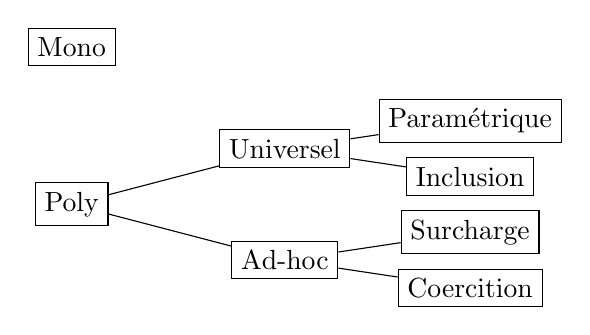
\begin{tikzpicture}
  [ ptype/.style={draw=black,shape=rectangle}
  , child/.style={ptype, xshift=2cm}
  , gen0/.style={       node distance=2cm}
  , gen1/.style={child, node distance=1cm}
  , gen2/.style={child, node distance=5mm}
  ]

  \node[ptype]                     (mono) {Mono};
  \node[ptype,below of=mono, gen0] (poly) {Poly};
  \node[above right of=poly, gen1] (univ)  {Universel};
  \node[above right of=univ, gen2] (param) {Paramétrique};
  \node[below right of=univ, gen2] (inclu) {Inclusion};
  \node[below right of=poly, gen1] (adho)  {Ad-hoc};
  \node[above right of=adho, gen2] (over)  {Surcharge};
  \node[below right of=adho, gen2] (coer)  {Coercition};

  \draw (poly) -- (univ);
  \draw (poly) -- (adho);

  \draw (univ) -- (param);
  \draw (univ) -- (inclu);

  \draw (adho) -- (over);
  \draw (adho) -- (coer);

      %node {Mono}
      %node {Poly}
          %node {Universal}
              %node {Param}
              %node {Inclusion}
          %node {Ad-Hoc}
              %node {Surcharge}
              %node {Coercition}

\end{tikzpicture}

\caption{Les différents types de polymorphisme.}
\label{fig:types-de-polymorphisme}
\end{figure}

\subsubsection{Monomorphisme}

Une première solution peut être de forcer des types concrets, c'est à dire
qu'une même fonction ne pourra s'appliquer qu'à un seul type de données.

Il est confortable pour le programmeur de n'avoir à écrire un algorithme qu'une
seule fois, indépendamment du type des éléments considérés.

Il existe deux grandes classes de systèmes de types introduisant du
polymorphisme.

\subsubsection{Polymorphisme universel}

% = {paramétrique, par inclusion}

Le polymorphisme est dit universel si toute fonction générique peut s'appliquer
à n'importe quel type.

\subsubsection{Polymorphisme ad-hoc}

% = {par surcharge, par coercition}

Le polymorphisme est \emph{ad-hoc} si les fonctions génériques ne peuvent
s'appliquer qu'à un ensemble de types prédéfini.

\subsubsection{Polymorphisme paramétrique}

\todo{Historique + citer le papier de Milner sur le polymorphisme}
\cite{Milner78}

\cite{PascalNoEscape}

\begin{figure}
  \insertcode{listappend.ml}
  \caption{Fonction de concaténation de listes en OCaml.}
  \label{fig:listappend}
\end{figure}

La fonction de la figure~\ref{fig:listappend} n'opère que sur la structure du type
liste (en utilisant ses constructeurs \texttt{{[}{]}} et \listcons ainsi que
le filtrage) : les éléments de \texttt{lx} et \texttt{ly} ne sont pas manipulés
à part pour les transférer dans le résultat.

Moralement, cette fonction est donc indépendante du type de données contenu dans
la liste : elle pourra agir sur des listes de n'importe quel type d'élément.

Plutôt qu'un type, on peut lui donner le \emph{schéma de types} suivant :

\[
  \textrm{append} : \forall a . a \textrm{list}
                             -> a \textrm{list}
                             -> a \textrm{list}
\]

C'est à dire que \texttt{append} peut être utilisé avec n'importe quel type
concret \texttt{a} en substituant les variables quantifiées (on parle d'
\emph{instanciation}).

\subsubsection{Polymorphisme par sous-typage}

\todo{héritage,sous-typage,classe,méthode,héritage multiple,late binding,Liskov}

Certains langages définissent la notion de sous-typage. C'est une relation
d'ordre partiel sur les types, qui modélise la relation "est un". Chaque
sous-classe peut redéfinir le comportement de chaque méthode de ses
superclasses.

\subsubsection{Polymorphisme par surcharge}

Considérons l'opération d'addition : \texttt{+}. On peut considérer que certains
types l'implémentent, et pas d'autres : ajouter deux flottants ou deux entiers a
du sens, mais pas ajouter deux pointeurs.

On dira que \texttt{+} est \emph{surchargé}. À chaque site d'appel, il faudra
\emph{résoudre la surcharge} pour déterminer quelle fonction appeler.

Cela rend l'inférence de types \todo{introduire l'inférence plus haut}
impossible dans le cas général, puisque certaines constructions sont ambigües.

\begin{figure}
  \insertcode{showread.hs}
  \caption{Cas d'ambigüité avec de la surcharge ad-hoc.}
  \label{fig:showread}
\end{figure}

Dans le code Haskell de la figure~\ref{fig:showread}, \texttt{show} peut
s'appliquer à toutes les valeurs de types "affichables" et renvoie une
représentation textuelle. \texttt{read} réalise le contraire avec les types
"lisibles".

Lorsqu'on compose ces deux fonctions, le type de la valeur intermédiaire est
capital puisqu'il détermine les instances de \texttt{show} et \texttt{read} à
utiliser.

\subsubsection{Polymorphisme par coercition}

\subsubsection{Polymorphisme d'ordre supérieur}

\begin{verbatim}
g f = (f true, f 2)
\end{verbatim}

\[
g : (\forall a . a -> a) -> (bool * int)
\]

Pas inférable (annotations nécessaires).

\subsection{Expressivité, garanties, types dépendants}

\section{Exemples}

\subsection{Faible dynamique : Perl}
\subsection{Faible statique : C}
\subsection{Fort dynamique : Python}
\subsection{Fort statique : OCaml}
\subsection{Fort statique à effets typés : Haskell}
\subsection{Theorem prover : Coq}

% vim: spelllang=fr
